\documentclass[10pt,twocolumn,letterpaper]{article}

\usepackage{cvpr} \usepackage{times} \usepackage{epsfig}
\usepackage{graphicx} \usepackage{amsmath} \usepackage{amssymb}

\graphicspath{ {figures/} }

\newenvironment{alt_enumerate}
{ \begin{enumerate}
		\setlength{\itemsep}{1pt}
		\setlength{\parskip}{1pt}
		\setlength{\parsep}{1pt} }
	{ \end{enumerate} }

% Include other packages here, before hyperref.

% If you comment hyperref and then uncomment it, you should delete
% egpaper.aux before re-running latex.  (Or just hit 'q' on the first latex
% run, let it finish, and you should be clear).
\usepackage[breaklinks=true,bookmarks=false]{hyperref}

\cvprfinalcopy % *** Uncomment this line for the final submission

\def\cvprPaperID{****} % *** Enter the CVPR Paper ID here
\def\httilde{\mbox{\tt\raisebox{-.5ex}{\symbol{126}}}}

% Pages are numbered in submission mode, and unnumbered in camera-ready
%\ifcvprfinal\pagestyle{empty}\fi
\setcounter{page}{1} \begin{document}

%%%%%%%%% TITLE
\title{Bird Audio Detection Challenge}

\author{
	Weilian Song, Tawfiq Salem, Nathan Jacobs\\ 
	University of Kentucky\\ 
	{\tt\small weilian.song@uky.edu, tawfiq.salem@uky.edu, jacobs@cs.uky.edu}
}

% TODO: Add Tawfiq in without messing up format

\maketitle
%\thispagestyle{empty}

%%%%%%%%% ABSTRACT
\begin{abstract}  

	Acoustic detection of birds in the wild is useful in many biological
	scenarios, including estimation of bird population and species-specific
	acoustic monitoring. Most current methods are either manual or
	semi-automatic, requiring labor-intensive processing/tuning. We hereby
	present three alternative methods, as part of the Bird Audio Detection
	Challenge, hosted by Queen Mary University of London. The first two
	methods are of our own submission, the third being the winning solution
	submitted by Thomas Grill. Each of said methods utilize deep neural
	networks for automatic, tuning-free bird presence detection: the first
	two emphasize network architectures, while the third utilizes multiple
	signal preprocessing techniques.

\end{abstract}

%%%%%%%%% BODY TEXT
\section{Introduction}

Much biological research relies on bird acoustic detection in audio signals,
as indicated by \cite{bad}. Over the recent years, a large amount of audio
data is recorded, but the bird detection methods are often manual or
semi-automatic, requiring intensive labor or tuning.

In response to the need for an automatic, tuning-free bird presence
detection algorithm, \textit{Bird Audio Detection Challenge} was created,
hosted by Queen Mary University of London and other universities. Three
datasets were released as part of the challenge, and teams across the world
compete for the best performance on the task of bird audio detection.

In section 2, we discuss some of the competition details, including the
datasets used, task description and the evaluation metrics. Section 3
presents three methods for bird acoustic detection, two of which are our
submission to the challenge, and the third one being the best performing
method submitted by Thomas Grill. Section 4 discusses some experiments and
techniques used to improve the peformance. Section 5 displays the
evaluation results of the three methods, and section 6 presents future
possible work that may result from this challenge.

%------------------------------------------------------------------------
\section{Competition Details}

The Bird Audio Detection Challenge is hosted by Queen Mary University of
London, in collaboration with the IEEE Signal Processing Society.

%-------------------------------------------------------------------------
\subsection{Task Description}

For the challenge, teams have to design a system that takes a short audio
clip, and returns a binary label denoting the presence/absence of any bird
species' sound. Teams are also encouraged to output a floating-point,
probability score in the range of 0 to 1 for evaluation purposes.

%-------------------------------------------------------------------------
\subsection{Datasets}

Three datasets are provided as part of the challenge.

% TODO: Should FreeSound be italicized?

\textbf{freefield1010:} 7,000 excerpts from field recordings around the
world, gathered by the FreeSound project.

\textbf{Warblr:} Crowd-sourced project with many smartphone recordings.
Very diverse in sound categories, even including human bird imitations.

% TODO: Should link to project be included?

\textbf{Chernobyl:} Part of TREE (Transfer-Exposure-Effects) research
project. Consists of ambient audio in the Chernobyl Exclusion Zone. 

Each dataset contains audio clips of roughly 10 seconds. For the challenge,
all datasets' audio files are provided, but only \textbf{freefield} and
\textbf{Warblr}'s labels are given. Held-out challenge dataset consists
primarily of the \textbf{Chernobyl} dataset, along with some from
\textbf{freefield} and \textbf{Warblr}.

%-------------------------------------------------------------------------
\subsection{Evaluation Metrics}

To evaluate the performance of a model, we use the standard "Area Under the
ROC Curve" method, also known as the AUC score.

%-------------------------------------------------------------------------
\section{Methodology}

Here we introduce three methods for bird acoustic detection, two of which
are proposed by us, and the third one being the best performing method by
Thomas Grill of University of Music and Performing Arts, Vienna. 

%-------------------------------------------------------------------------
\subsection{Data preparation}

All individual audio clips are 10 seconds, mono at 44,100 Hz, which gives us
441,000 frames of audio. We divide all frames by 32,768 to convert values of
individual frames to between -1 and 1, and randomly crop out 400,000
continuous frames, resulting in a one-dimensional vector with length 400,000
as our input to the network.

%-------------------------------------------------------------------------
\subsection{Method 1}

% TODO: Weird spacing issue in first and second sentence

Our first method resembles basic characteristics of SoundNet by Aytar et
al.\cite{soundnet} and Residual Net by He et al.\cite{residual_net}. The
network is fully convolutional, with one-dimensional convolutions followed
by non-linear (ReLU) layers. This network is suitable for audio
signals, as it is invariant to translation and allows stacking of
convolutional layers for detecting high-level features.

This network also has shortcuts from earlier layers of the network to later
stages, allowing easier gradient back-propagation to early layers of the
network. See Figure 1 for network details.

\begin{figure}[t]
	\centering
	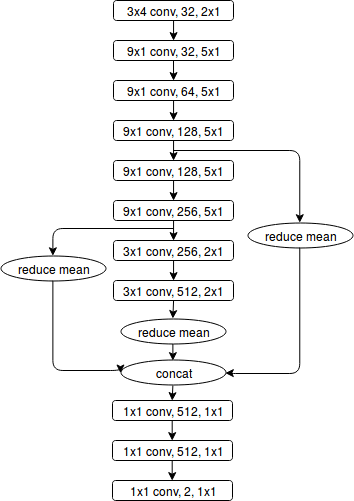
\includegraphics[width=0.5\textwidth]{v5_diagram}
	\caption{Network v5 Architecture. Content within convolutional blocks
	refers to kernel size, number of filters, and stride size}
\end{figure}

%------------------------------------------------------------------------

\subsection{Method 2}

Our second method utilizes a series of pooling and convolutional layers to
extract features from the input audio at different temporal resolutions,
and concatenate them before some final convolutional layers.

This network can be divided into three stages. In the first stage, we first
create two copies of the input, one reshaped to 100,000 by 4, and the other
reshaped to 200,000 by 2. \(x_{100,000*4}\) is then passed through a single
convolutional layer while \(x_{200,000*2}\) is passed through a series of 5
averaging pooling layers, followed by a convolutional layer at the end of
each pooling layer. Note here that the input of one pooling layer is the
output of the previous pooling layer; the outputs of the convolutional
layers serve as features extracted at input of different temporal
resolution.

In the second stage, we combine the outputs of the 6 convolutional layers
in stage 1 into one feature vector. First, we find the maximum for each
convolutional output. We denote them as the energy for each convolutional
layer. We then concatenate them with their corresponding convolutional
output, pass each concatenated feature vector through a pooling layer of
specified size, and concatenate all 6 pooled feature vectors. Due to
different lengths of output from the 6 convolutional layers in stage 1, we
pass them through pooling layers of different sizes to ensure that they are
of the same dimension for concatenation.

In the final stage, we pass the output from stage 2 through a batch
normalization layer, followed by 7 additional convolutional layers, with a
\(max()\) operation between the 4th and 5th layer. Final output is then
flattened into size (1,2), ready to be used in a softmax classification
loss function.

\begin{figure*}
	\centering
	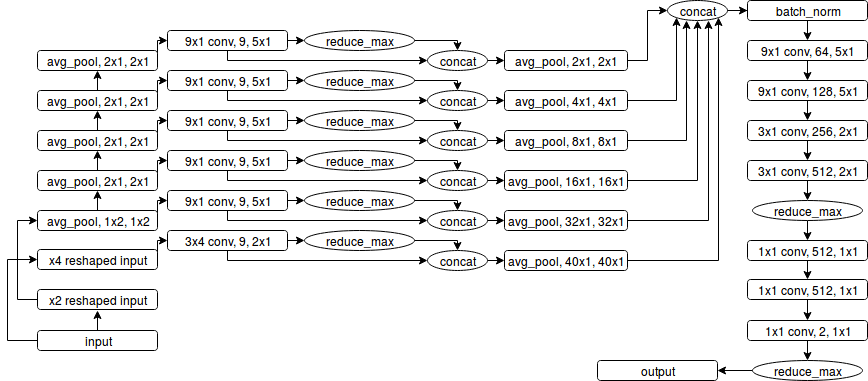
\includegraphics[width=\textwidth]{v8_diagram}
	\caption{Network v8 Architecture. Content of convolutional blocks refer
	to kernel size, number of filters, and stride size. Content of avgpool
	blocks refer to kernel size and stride size.}
\end{figure*}

%------------------------------------------------------------------------
\subsection{Method 3}

This method is the winning algorithm to the challenge, submitted by Thomas
Grill. The neural network uses processed spectrograms of audio clips as
input, instead of a one-dimensional vector of signals. The network consists
of 4 convolutional layers with pooling, and 2 dense layers. Multiple signal
pre-processing techniques are used, including silence/noise trimming, and a
different data augmentation technique involving shifting the spectrograms
in time and frequency.  Pseudo-labeling and bagging techniques are also
deployed, which we will discuss in section 4.

%------------------------------------------------------------------------
\section{Experiments}

During our development, we experimented with various pre- and
post-processing techniques, as well as some training strategies.

%------------------------------------------------------------------------
\subsection{Implementation Details}

The given labeled data from both datasets is split into 10 folds. Within
each fold, the number of positive(bird present) and negative(bird absent)
samples are balanced. During training, the number of samples loaded from
each datasets are also balanced, to ensure no bias.

For in-house testing, 9 folds are used for training and 1 fold for testing.
For submission, all 10 folds are used for training.

For method 1 and 2, we implemented them in python with Tensorflow machine
learning library. We trained from scratch, with learning rate of 0.03,
learning rate decay by a factor of 0.1 every 40,000 iterations, and a total
of 300,000 iterations.

For method 3, a brief description and code base is available online
at\cite{winning_blog}.

% TODO: How to include code base link?

%------------------------------------------------------------------------
\subsection{Data Augmentation}

We deploy data augmentation as our only pre-processing technique for method
1 and 2. Given one base sound clip, positive or negative (bird
present/absent), and another negative sound clip, we concatenate them along
the y-axis, with the base clip weighted by a factor \(r\) between 0.25 and
1, and the negative sound clip weighted by a factor \(1-r\). Thus we have:
\begin{equation}
	x_{augmented}=r*x_{base} + (1-r)*x_{negative}
\end{equation}
If \(r\) equals to 1, then there would be no augmentation, and if \(r\)
equals to 0.25, only 25\% of the base sound clip will be preserved. We
sample \(r\) on a positively skewed interval (0.25,1) to ensure bird sounds
in positive labels are not diminished.

Label for the augmented clip will remain the same as the base clip, as the
augmentation is an \textit{or} process, preserving the original label when 
"\textit{or}-ed" with a negative label.

%------------------------------------------------------------------------
\subsection{Reducing capacity}

One main difficulty we faced was the small size of training data. With no
regularization, our networks consistently over-fit to the training data,
performed nearly perfectly on training and our own held-out test data, but
performed poorly on the challenge data. To compensate for this, we reduced
the capacity of our models by reducing the number of filters for each
convolutional layer. We did so until the network could not perform
perfectly on the training and testing data.

%------------------------------------------------------------------------
\subsection{Prediction Bagging}

This post-processing technique averages prediction scores from many
sessions. Due to the random cropping of audio signals during the data
loading phase, different evaluation of the same audio clip will yield
slightly different results. Therefore we predicted 100 sets of scores for the
held-out challenge dataset, and averaged them to capture the true scores for
submission.

For method 3, instead of averaging sets of output scores from the same
model, different models' outputs were averaged. Please refer to Grill's
code base\cite{winning_blog} for more details.

%------------------------------------------------------------------------
\subsection{Domain Confusion}

% TODO Consult with Dr. Jacobs on whether this should be mentioned or not

This training strategy addresses the issue of dataset bias. It is apparent
that the three given datasets have disjoint sound domains. In addition,
within each dataset, data is skewed either towards mostly positive samples
or mostly negative ones. During training, it is very likely that the
network will cheat by identifying which dataset the clip is from, and make
its prediction based off of that information. In response, we take the
audio features near the end of the network, pass it through another
convolutional layer, and... 

%------------------------------------------------------------------------
\subsection{Pseudo Labeling}

This technique is used by many contestants and was attempted by us. The
assumption is that high-confidence predictions on the held-out challenge
dataset are accurate enough to be used as extra data for retraining or
fine-tuning. Basic procedures are:

\begin{alt_enumerate}
	\item{Train a model with only labeled data}
	\item{Predict scores of the held-out challenge dataset}
	\item{Find threshold \(r\) such that predictions within range\\
		\(0<r \cup (1-r)<1\) are accurate enough}
	\item{Add all predictions within threshold, and retrain or fine-tune
		network}
\end{alt_enumerate}

\(r\) can be obtained through manual spot-checking of the predictions. Too
much time spent on finding the threshold will defeat the purpose of the
challenge.

%------------------------------------------------------------------------
\section{Results}

Below are the final AUC scores for each of the 3 methods:\\

\begin{tabular}{ |p{2cm}|p{2cm}|p{2cm}|p{2cm}| }
	\hline
	\multicolumn{2}{|c|}{AUC Scores}\\
	\hline
	Method & AUC Score\\
	\hline
	Method 1 & 77.9\\
	Method 2 & 78.8\\
	Method 3 & 88.7\\
	\hline
\end{tabular}

%------------------------------------------------------------------------
\section{Future Work}

For methods 1 and 2, no signal pre-processing techniques were deployed,
resulting in very noisy inputs to our network. It will be interesting to
find out if pre-processing will aid the prediction accuracy of our two
networks.

%------------------------------------------------------------------------
\section{Conclusion}

Bird acoustic detection is an important task for many biological
applications, but the massive amount of data available makes it difficult
to extract any useful information from it. The Bird Audio Detection
challenge has advanced this field greatly--many excellent automatic,
tuning-free bird acoustic detection algorithms are introduced.  We
presented three methods, the first two with a focus on unique network
architectures, and the third one as the embodiment of many years of machine
listening research.  Many topics are still open for research, including
numerous tasks that already have a solution, but can only be achieved
through manual or labor intensive annotation.

%------------------------------------------------------------------------

{\small \bibliographystyle{ieee} \bibliography{biblio} }

\end{document}
